%%%%%%%%%%%%%%%%%%%%%%%%%%%%%%%%%%%%%%%%%
% Structured General Purpose Assignment
% LaTeX Template
%
% This template has been downloaded from:
% http://www.latextemplates.com
%
% Original author:
% Ted Pavlic (http://www.tedpavlic.com)
%
% Note:
% The \lipsum[#] commands throughout this template generate dummy text
% to fill the template out. These commands should all be removed when 
% writing assignment content.
%
%%%%%%%%%%%%%%%%%%%%%%%%%%%%%%%%%%%%%%%%%

%----------------------------------------------------------------------------------------
%	PACKAGES AND OTHER DOCUMENT CONFIGURATIONS
%----------------------------------------------------------------------------------------

\documentclass{article}

\usepackage{fancyhdr} % Required for custom headers
\usepackage{lastpage} % Required to determine the last page for the footer
\usepackage{extramarks} % Required for headers and footers
\usepackage{graphicx} % Required to insert images
\usepackage{caption}
\usepackage{float}
\usepackage{url}
\usepackage{subcaption}


% Margins
\topmargin=-0.45in
\evensidemargin=0in
\oddsidemargin=0in
\textwidth=6.5in
\textheight=9.0in
\headsep=0.25in 


\linespread{1.1} % Line spacing

% Set up the header and footer
\pagestyle{fancy}
\lhead{\hmwkAuthorName} % Top left header
\chead{\hmwkClass\ \hmwkTitle} % Top center header
\rhead{\firstxmark} % Top right header
\lfoot{\lastxmark} % Bottom left footer
\cfoot{} % Bottom center footer
\rfoot{Page\ \thepage\ of\ \pageref{LastPage}} % Bottom right footer
\renewcommand\headrulewidth{0.4pt} % Size of the header rule
\renewcommand\footrulewidth{0.4pt} % Size of the footer rule

\setlength\parindent{0pt} % Removes all indentation from paragraphs

%----------------------------------------------------------------------------------------
%	DOCUMENT STRUCTURE COMMANDS
%	Skip this unless you know what you're doing
%----------------------------------------------------------------------------------------

% Header and footer for when a page split occurs within a problem environment
\newcommand{\enterProblemHeader}[1]{
\nobreak\extramarks{#1}{#1 continued on next page\ldots}\nobreak
\nobreak\extramarks{#1 (continued)}{#1 continued on next page\ldots}\nobreak
}

% Header and footer for when a page split occurs between problem environments
\newcommand{\exitProblemHeader}[1]{
\nobreak\extramarks{#1 (continued)}{#1 continued on next page\ldots}\nobreak
\nobreak\extramarks{#1}{}\nobreak
}

\setcounter{secnumdepth}{0} % Removes default section numbers
\newcounter{homeworkProblemCounter} % Creates a counter to keep track of the number of problems

\newcommand{\homeworkProblemName}{}
\newenvironment{homeworkProblem}[1][Problem \arabic{homeworkProblemCounter}]{ % Makes a new environment called homeworkProblem which takes 1 argument (custom name) but the default is "Problem #"
\stepcounter{homeworkProblemCounter} % Increase counter for number of problems
\renewcommand{\homeworkProblemName}{#1} % Assign \homeworkProblemName the name of the problem
\section{\homeworkProblemName} % Make a section in the document with the custom problem count
\enterProblemHeader{\homeworkProblemName} % Header and footer within the environment
}{
\exitProblemHeader{\homeworkProblemName} % Header and footer after the environment
}

\newcommand{\problemAnswer}[1]{ % Defines the problem answer command with the content as the only argument
\noindent\framebox[\columnwidth][c]{\begin{minipage}{0.98\columnwidth}#1\end{minipage}} % Makes the box around the problem answer and puts the content inside
}

\newcommand{\homeworkSectionName}{}
\newenvironment{homeworkSection}[1]{ % New environment for sections within homework problems, takes 1 argument - the name of the section
\renewcommand{\homeworkSectionName}{#1} % Assign \homeworkSectionName to the name of the section from the environment argument
\subsection{\homeworkSectionName} % Make a subsection with the custom name of the subsection
\enterProblemHeader{\homeworkProblemName\ [\homeworkSectionName]} % Header and footer within the environment
}{
\enterProblemHeader{\homeworkProblemName} % Header and footer after the environment
}
   
%----------------------------------------------------------------------------------------
%	NAME AND CLASS SECTION
%----------------------------------------------------------------------------------------

\newcommand{\hmwkTitle}{"Where Have I Been?" - Languages Comparison} % Assignment title
\newcommand{\hmwkDueDate}{Friday,\ April\ 11,\ 2014} % Due date
\newcommand{\hmwkClass}{CS\ 22510} % Course/class
\newcommand{\hmwkAuthorName}{James Euesden - jee22} % Your name

%----------------------------------------------------------------------------------------
%	TITLE PAGE
%----------------------------------------------------------------------------------------

\title{
\vspace{2in}
\textmd{\textbf{\hmwkClass:\ \hmwkTitle}}\\
\normalsize\vspace{0.1in}\small{Due\ on\ \hmwkDueDate}\\
\vspace{3in}
}

\author{\textbf{\hmwkAuthorName}}
\date{} % Insert date here if you want it to appear below your name

%----------------------------------------------------------------------------------------

\setlength\parindent{24pt}

\begin{document}

\maketitle

%----------------------------------------------------------------------------------------
%	TABLE OF CONTENTS
%----------------------------------------------------------------------------------------

%\setcounter{tocdepth}{1} % Uncomment this line if you don't want subsections listed in the ToC

\newpage
\tableofcontents
\newpage

%----------------------------------------------------------------------------------------
%	INTRODUCTION
%----------------------------------------------------------------------------------------

% To have just one problem per page, simply put a \clearpage after each problem

\section{Introduction}
This document is the second part (Assignment 2\cite{assignment2}) of the "Where have I been?" assignment. In this report, I will discuss the languages and my experiences with them. While the first part (Assignment 1\cite{assignment1}) was about the programming for GPS Processing, this is about the differences between the languages and my experiences with them while writing the applications. What I found useful or difficult, any libraries I may have chosen to use, and what language I felt was best suited to the task.


%----------------------------------------------------------------------------------------
%	LANGUAGE COMPARISONS
%----------------------------------------------------------------------------------------

\section{Language Comparisons}

The amount of code between each language was rather similar. I used GitHub\cite{github} to keep track of my code and the versions of it as I completed part one of the assignment. One of the benefits of doing this was that it provided a great break down of how much percentage of the repo was taken up by the different languages (screenshot taken before this document was added to the repository):

\begin{figure}[h!]
  \centering
    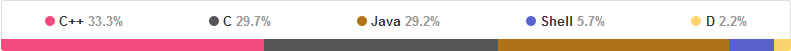
\includegraphics[width=1\textwidth]{img/percentages}
  \caption{The percentage of languages for part 1.}
\end{figure}

The figure shows that the amount of code for each language was very similar. I feel the reason C++ has more code than the other two may be due to each class having a Constructor, a Destructor and a Copy Constructor, whether they were used or not. With this in mind, it should be apparent that my writing of the application in each language was very similar, and while one particular section in one language may take more code than another, that same language may do something much simpler than the others.

An example would be the file operations in Java vs C, where it takes more for C to handle getting the data out of the file and char arrays than in Java. Opposite to this, my C program handles date and time much easier and with less code than that used in Java. Overall, I found the simplicity of C and C++ helped me in writing the code in the most simplest way I could think of.

\subsubsection{Code Clarity}

The code for all three applications is quite clear in it's operations, and I feel this is down to the way I wrote the code and comments. Through the use of good naming conventions and meaningful variables/methods/functions, the flow of each application can be followed and understood through the names of the components. It can get a little unclear in some aspects, such as setting the Latitude and Longitude from a char array in C, but any obscurities can be cleared up with comments.

Each language has it's own syntax and quirks when it comes to the way that applications should be written. In this case, the general logic of the applications was the same and any language-specific quirks weren't too difficult for me to understand when programming, or to understand when reading back over the code after some time of not working with it.
\begin{figure}[H]
        \centering
        \begin{subfigure}[b]{0.4\textwidth}
                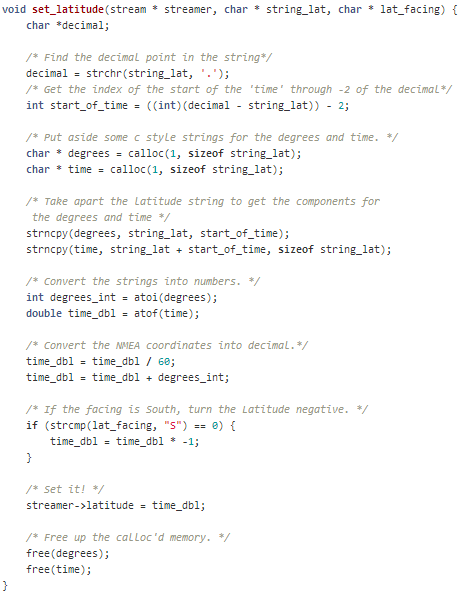
\includegraphics[width=\textwidth]{img/latitude}
                \caption{An excerpt from my C application: Setting Latitude from a char array and converting it from NMEA to decimal.}
                \label{fig:latc}
        \end{subfigure}%
        ~ %add desired spacing between images, e. g. ~, \quad, \qquad etc.
          %(or a blank line to force the subfigure onto a new line)
        \begin{subfigure}[b]{0.5\textwidth}
                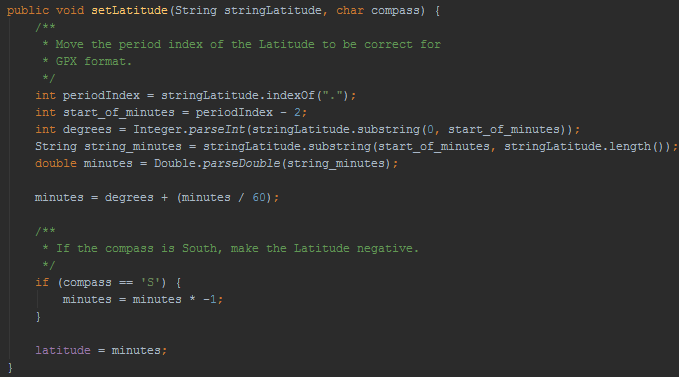
\includegraphics[width=\textwidth]{img/latitudejava}
                \caption{An excerpt from my Java application: Setting Latitude from a String and converting it from NMEA to decimal.}
                \label{fig:latjava}
        \end{subfigure}
        \caption{The difference between Java and C, in code clarity when setting the Latitude.}\label{fig:latitudediff}
\end{figure}

\subsubsection{File Operations}

In all three languages, the file input and output was relatively simple and similar. With Java, I had a slight difference in that on every update of a timestamp I output the XML into a StringBuilder, and then output the full String at the very end of the application. While with the C and C++, I output directly to the file when a timestamp was updated. This was made very easy through the use of pointers to the FILE, and keeping a reference to the class for the file operations. All three languages, while different, were relatively helpful with reading in from a file.


\subsubsection{Data Accessibility \& Manipulation}

With Java and C++ having objects rather than simple source files with functions and variables, I was able to put a variable as private, and restrict access to it from outside of the class except through the use of defined getters and setters. Data is relatively easy to access in C, and it isn't as secure as setting something as private. In this regard, C lets itself down in that it is not 'open for extension, closed for modification' when data is in a struct that has been included in a file. This can lead to future developers circumventing the way that the original programmer intended data to be accessed, should this application be built upon in the future.

In terms of manipulating the data, there were generally no problems. The only issues I encountered were in C and C++, when I had to remember to set values to something before allowing them to be used/compared with something, in the off chance that they had not been initialized to 0 or null, and instead contained data from elsewhere. While not a huge hinderence to program, it sometimes made debugging provide very interesting results if I had forgotten to do this.

\subsubsection{Memory Allocation}

It was useful to have the 'garbage collection' in Java, saving me from having to use free() and delete(). In C and C++ I had to trace the bits of memory to where they should correctly end and remove them appropriately, without accidentally causing the application's memory to lose it's integrity with a double free situation. On the other hand, the freedom of allocating and freeing memory gave me much more control over how data was stored in the applications. While the applications were only small and so didn't take up too much memory, it is something that I will be keeping in mind for future applications where I have a choice of language and want to be memory space conscious.

\subsubsection{Date \& Time}

For both C and C++ I used the 'time' library\cite{ctime}, and for Java used the Calendar\cite{calendar} class. I found the Calendar class cumbersome to use and in some ways hindered my programming. On the other hand, using the time library was perfect for comparing timestamps, creating new timestamps from sentence data and even updating a timestamp with new sentence data without a date. 

When programming in Java and using Calendar, updating the date and time provided by a sentence with both date and time was fine. However, when it came to updating a time without a provided date, it became much more difficult to do and I spent a good while writing and re-writing code to use an older Calendar object to create a new one with the updated time.

In C and C++, this was simple to do by turning the most recent time\_t struct back into a tm struct, updating the values and then using mktime() to get it back to time\_t. While the process with Calendar ended up quite similar, I found that I had trouble getting the time to be correct, with milliseconds assigned randomly, and needing to use .clone() to get correct values for the date, which slowed down my progress when writing the Java application.




%-------------------------------------------- Compare/Contrast. Amount of code written, the clarity of code, any features that helped/hindered the representation of my solution.



%----------------------------------------------------------------------------------------
%	LIBRARIES
%----------------------------------------------------------------------------------------

\section{Libraries}

I chose not to use any libraries outside of those provided with the standard API of the native languages. Below are some libraries that I could have used, why they could have been useful, and why I didn't use them.

\subsubsection{NMEA parsing}
For all three languages there are libraries that I could have used in order to parse the NMEA sentences into data, without having to dissect and extract the data\cite{nmeajava}\cite{nmeacplusplus} myself. However, I chose not to use any of these. My main reason for this is that I wanted to understand the sentences myself, and to only extract the data I wanted and then discard them, rather than extract all data from the sentences. On a larger project that intended to use the majority of data from the NMEA sentences, I would look into using one of these open source libraries to save time. For my own assignment in my own work, I felt that it was acceptable to not use these.

\subsubsection{C++: Boost}
There is a library for C++ called Boost\cite{boost}. This library provides many useful functions for C++ that aren't in the native language. A number of these could be have been useful for manipulating strings, and saved me time and code. However, as with the NMEA 0813 sentences, for an assignment of this size I would rather use my own code and work through the problem to better my understanding of C++. Boost is a useful library that I will remember for future projects where their functions may be invaluable in saving me time and effort.

\subsubsection{XML Builders}
While not an additional library, Java has the use for classes such as DocumentBuilder\cite{javaxml}\cite{documentbuilder}, which can XML tag a file (UTF-8) for us. Again, I chose not to use this, and provided my own methods for putting tags around the data. This is partially because of tags such as "<wpt lat="" lon=""> where it is a tag built up of multiple components I found easier to do myself, and also because of the size and amount of XML tags being output being so little. If the applications were required to output a larger variety of XML tags, I may have found it useful to find XML Builders. For what the problem consisted of, I felt it was easy enough to do it myself, and to further my understanding of building XML files in my programming.

%-------------------------------------------- What Libraries could I have used? How could they have helped?

%----------------------------------------------------------------------------------------
%	CONCLUSION
%----------------------------------------------------------------------------------------


\section{Conclusion \& Suitability}
In terms of what language is best suited for writing this application, I would say that a lot of it comes down to personal opinion. I found all three languages had their challenges or parts that aided me, and so each of them is acceptably suitable for this process. 

However, if I had to choose, I felt that C++  was the most suitable for my implementation. My justification for this is that I found it the easiest and quickest to write in. The methods are all relatively simplistic. it has the simplicity of C, while providing the bonuses of Object Oriented programming. The fact that C++ has access to it's own libraries and functions, while also having access to those provided in C, made C++ a joy to write the application in with ease. Adding to this that there are libraries like Boost and NMEA parsers, and it becomes clear to me that C++ is perhaps the most suited for this application out of all in my opinion.

%----------------------------------------------------------------------------------------
\clearpage

%----------------------------------------------------------------------------------------
%	REFERENCES
%----------------------------------------------------------------------------------------

\begin{thebibliography}{10}

\bibitem{assignment2} F. Labrosse and J. Bell, "Where have I been? - languages comparison", CS22510 assignment 2, February 24 2014

\bibitem{assignment1} F. Labrosse and J. Bell, "Where have I been? - processing GPS data", CS22510 assignment 1 - Version 2, March 18 2014 (original: February 24 2014)

\bibitem{github} coderGhast - James, {\em GitHub},[online], https://github.com/coderGhast (Accessed:27/03/2014)

\bibitem{ctime} ctime - cppreference, {\em cppreference},[online], http://en.cppreference.com/w/c/chrono/ctime (Accessed:27/03/2014)

\bibitem{calendar} Calendar (Java Platform SE 7), {\em docs.oracle},[online], http://docs.oracle.com/javase/7/docs/api/java/ util/Calendar.html (Accessed:27/03/2014)

\bibitem{nmeajava} NMEA Java library, {\em nmealib.sourceforge},[online], http://nmealib.sourceforge.net/ (Accessed:27/03/2014)

\bibitem{nmeacplusplus} NMEA library, {\em nmea.sourceforge},[online], http://nmea.sourceforge.net/ (Accessed:27/03/2014)

\bibitem{boost} Boost C++ Libraries, {\em boost},[online], http://www.boost.org/ (Accessed:27/03/2014)

\bibitem{javaxmlr} How to create XML file in Java - (DOM parser), {\em mkyong},[online], http://www.mkyong.com/java/how-to-create-xml-file-in-java-dom/ (Accessed:27/03/2014)

\bibitem{documentbuilder} DocumentBuilder (Java Platform SE 7), {\em docs.oracle},[online], http://docs.oracle.com/javase/7/docs/api/ javax/xml/parsers/DocumentBuilder.html (Accessed:27/03/2014)

\end{thebibliography}


\end{document}


